\documentclass{beamer}[10pt]
\usepackage{listings}
\usepackage{xcolor}

\definecolor{codegreen}{rgb}{0,0.6,0}
\definecolor{codegray}{rgb}{0.5,0.5,0.5}
\definecolor{codepurple}{rgb}{0.58,0,0.82}
\definecolor{backcolour}{rgb}{0.95,0.95,0.92}

\lstdefinestyle{mystyle}{
    backgroundcolor=\color{backcolour},   
    commentstyle=\color{codegreen},
    keywordstyle=\color{magenta},
    numberstyle=\tiny\color{codegray},
    stringstyle=\color{codepurple},
    basicstyle=\ttfamily\footnotesize,
    breakatwhitespace=false,         
    breaklines=true,                 
    captionpos=b,                    
    keepspaces=true,                 
    numbers=left,                    
    numbersep=5pt,                  
    showspaces=false,                
    showstringspaces=false,
    showtabs=false,                  
    tabsize=2
}

\lstset{style=mystyle}


\usetheme{Madrid}
\setbeamertemplate{navigation symbols}{}
\title[DeAnonTor]{DeAnonimize TOR Network}
\subtitle[]{whit fingerprinting analisys}
\author[Paola Guarasci]{Paola Guarasci}
% \institute[Unical]{Università della Calabria}
\date[07/2022]{July 2022}

% Description of the specific BCP (BEST CURRENT PRACTICE)/CWE/CVE number, or in general, of the project topic.
% Whenever applicable, description of the technological context of the assigned BCP/CWE/CVE/General topic, including criticism, if any (e.g. show that a given BCP is outdated and why, etc.)
% Examples (for a CWE, an example can consist in a specific CVE)

\begin{document}
\frame{\titlepage}

\begin{frame}
  \frametitle{Descrizione del progetto}
  Il progetto prevede la deanonimizzazione di un utente TOR a partire dalle fingerprint dei siti web visitati.
  \\In particolare e' possibile creare una correlazione tra le risorse e il traffico generato per la loro fruizione.
  \\La correlazione avviene facendo un'analisi statistica dei pacchetti TCP che vengono viaggiano attraverso la rete TOR.\@
  Il primo paper e' del 2013 e riporta uno studio condotto in closed-world su un campione di 750 siti web. In particolare si parla di pagine, non di siti interi.
\end{frame}

\begin{frame}
  \frametitle{Aspetti tecnici}
  Un attacco fingerprint puo' essere realizzato in ambiente chiuso e in ambiente aperto. In ambiente chiuso Darth e' ha conoscenza di tutti i siti web visitati dall'utente TOR, in ambiente aperto invece il Alice e Bob possono visitare ogni sito web esistente.
  Per realizzare questo progetto e' stato creato un ambiente chiuso, in GNS3, in cui il possibile ventaglio dei siti visitabilio e' limitato a 5.
  Nel blog del progetto TOR si trova una \href{https://blog.torproject.org/critique-website-traffic-fingerprinting-attacks/}{descrizione}  piu' dettagliata di questo tipo di attacco.
  Un attacco di questo tipo prevede che Darth si posizione tra il client e il primo relay del circuito, il Guard relay. Potrebbe ad esempio essere sfruttato da un ISP per censurare alcuni contenuti.
  \\ Le informazioni analizzare sono: lunghezza dei pacchetti, timing.
\end{frame}

\begin{frame}
  \frametitle{Elenco Metodologie DeAnonimize}
  Le metodologie di attacco sono le seguenti:
  \begin{itemize}
    \item Sniffing tra client e ISP
    \item Sniffing tra client e ISP e tra WebServer e ISP
  \end{itemize}
\end{frame}

\begin{frame}
  \frametitle{Descrizione Demo}
  La medotologia scelta per la demo e' lo Sniffing tra Client e ISP.\@
  \\ Questo tipo di attacco consente di comprendere quali website sta visitando il nostro target, anche se il traffico passa attraverso una rete TOR.\@ Il punto principale dell'attacco e' l'analisi dei pacchetti.\@
  \\ Quindi facendo inferenze su dimensione, direzione e quantita' dei pacchetti TCP (le fingerprint) si puo' ipotizzare a quale sito (noto) appartiene il traffico generato.
\end{frame}

\begin{frame}
  \frametitle{Laboratorio}
  Il laboratio GNS3 realizzato per questo progetto conta un totale di 10 host Debian 11 emulati con QEMU e Tor 0.4.5.10, 3 router Cisco 7200 e 4 switch Cisco 3745.
  \begin{figure}
    \centering
    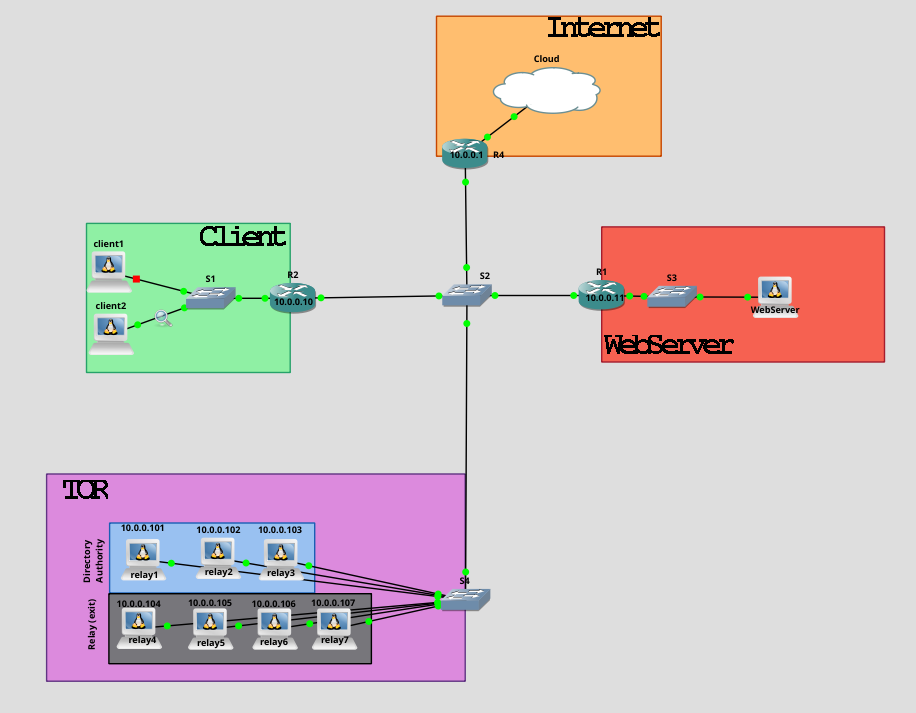
\includegraphics[width=0.60\textwidth]{../img/topology.png}
  \end{figure}

\end{frame}

\begin{frame}
  \frametitle{Rete Tor}
  La rete Tor e' stata creata partendo dalle configurazioni suggerite dal simulatore di reti Tor private (Chutney). Al suo interno la rete e' divisa in:
  \begin{itemize}
    \item 3 DA (Relay autoritativi)
    \item 4 Relay di uscita
  \end{itemize}
  Ognuno di questi host ha un accesso diretto alla rete interna del laboratorio, per simulare il piu' possibile il fatto che presumibilmente in un contesto reale questi server dispongono di un ip pubblico.
  La configurazione con 3 directory autority e' conseguenza di alcuni espreimenti in cui la rete non funzionava a dovere e ho poi compreso che le reti Tor necessitano di almeno 3 host auth/mid/exit per creare le rotte.
  In questi 3 elementi pero' ogni host non include se stesso. Questa configurazione 3+4 e' per me la configurazione minima funzionante.
\end{frame}


\begin{frame}
  \frametitle{Test della rete}
  \begin{figure}
    \centering
    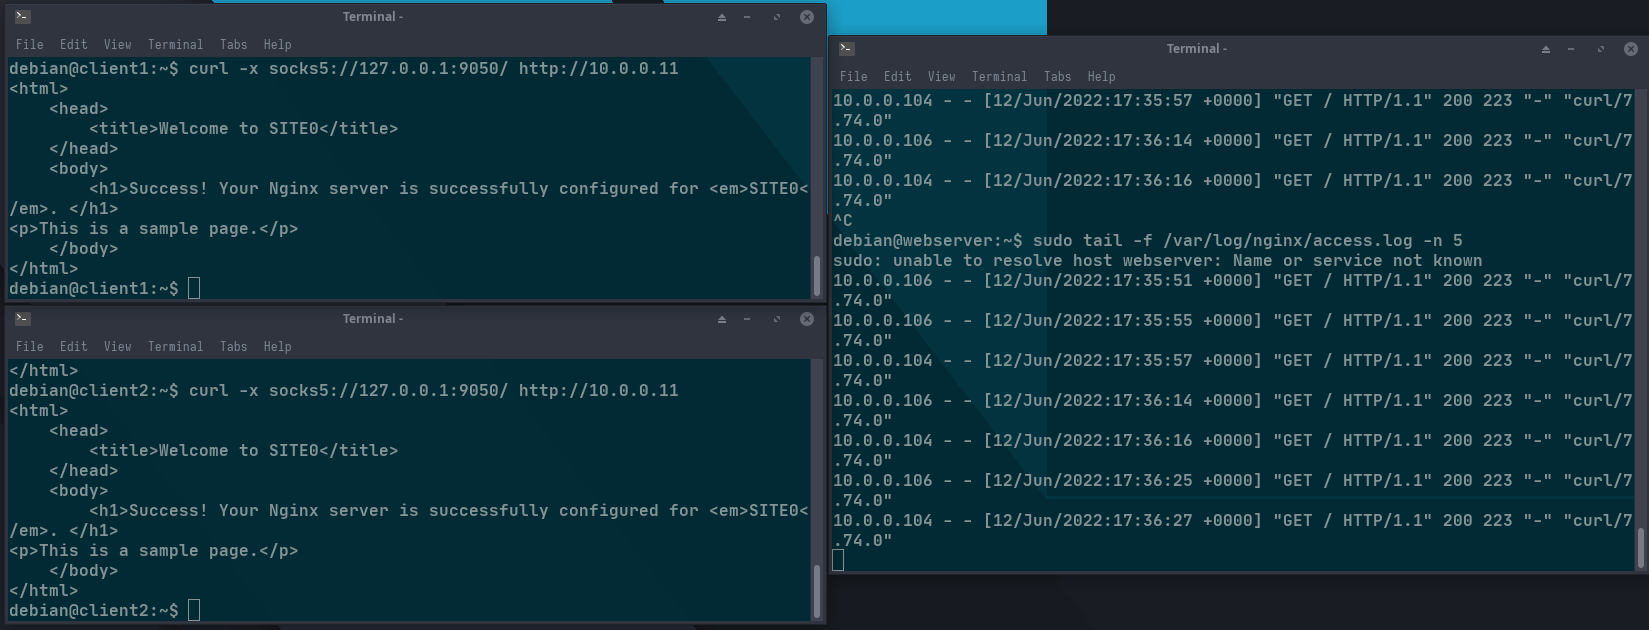
\includegraphics[width=0.851\textwidth]{../img/terminali_2.png}
  \end{figure}
\end{frame}

\begin{frame}
  \frametitle{Esecuzione di un attacco}
  \begin{itemize}
    \item Wireshark in ascolto su link client-isp
    \item Visita di un sito random da parte del client
    \item Generazione delle fingerprint (python, su macchina host, da cattura in csv)
    \item Confronto tra grafico random e grafici noti
  \end{itemize}
\end{frame}

\begin{frame}
  \frametitle{Confronti 1}
  \begin{columns}[T]
    \begin{column}{0.33\textwidth}
      \begin{center}
        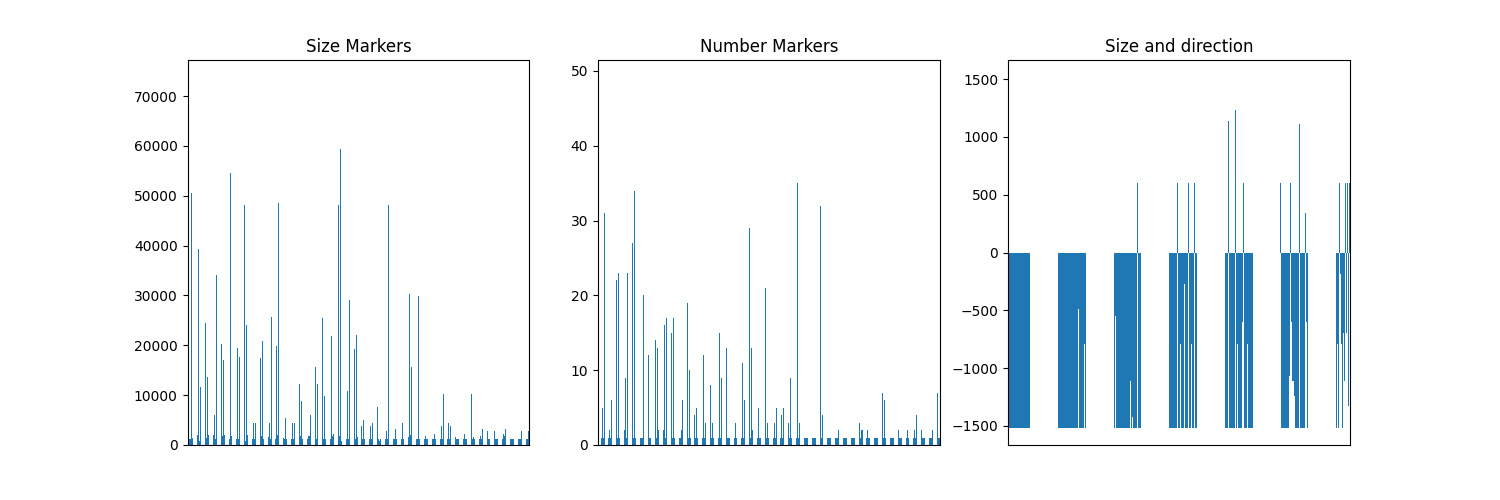
\includegraphics[width=\textwidth]{../img/ansa-figure.png}
        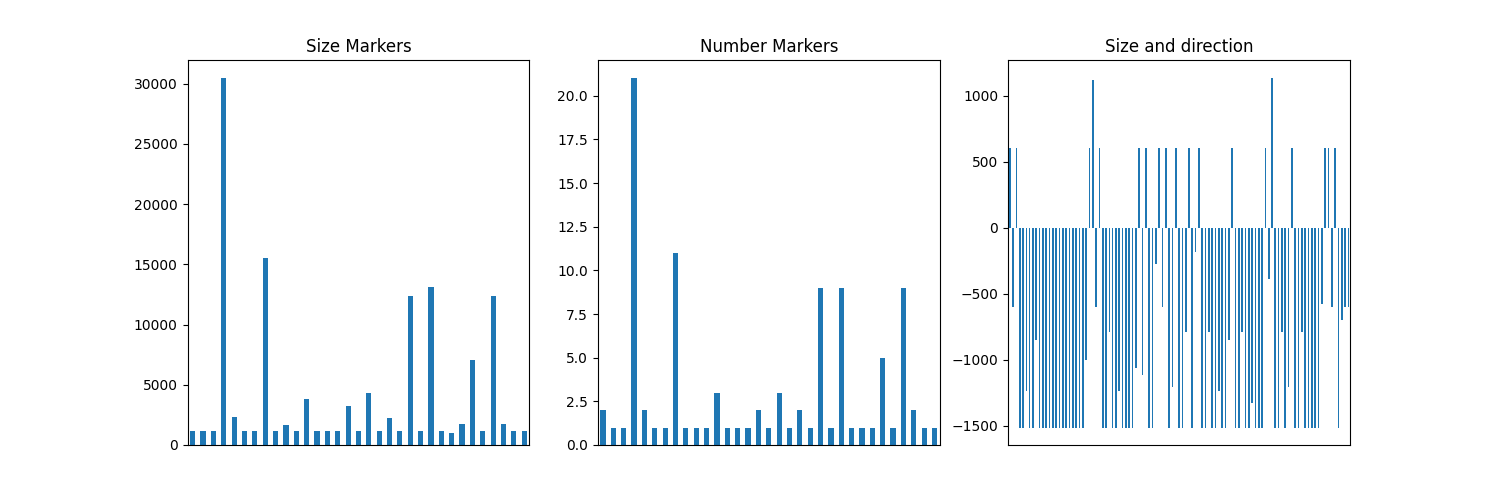
\includegraphics[width=\textwidth]{../img/archlinux-figure.png}
      \end{center}
    \end{column}
    \begin{column}{0.33\textwidth}
      \begin{center}
        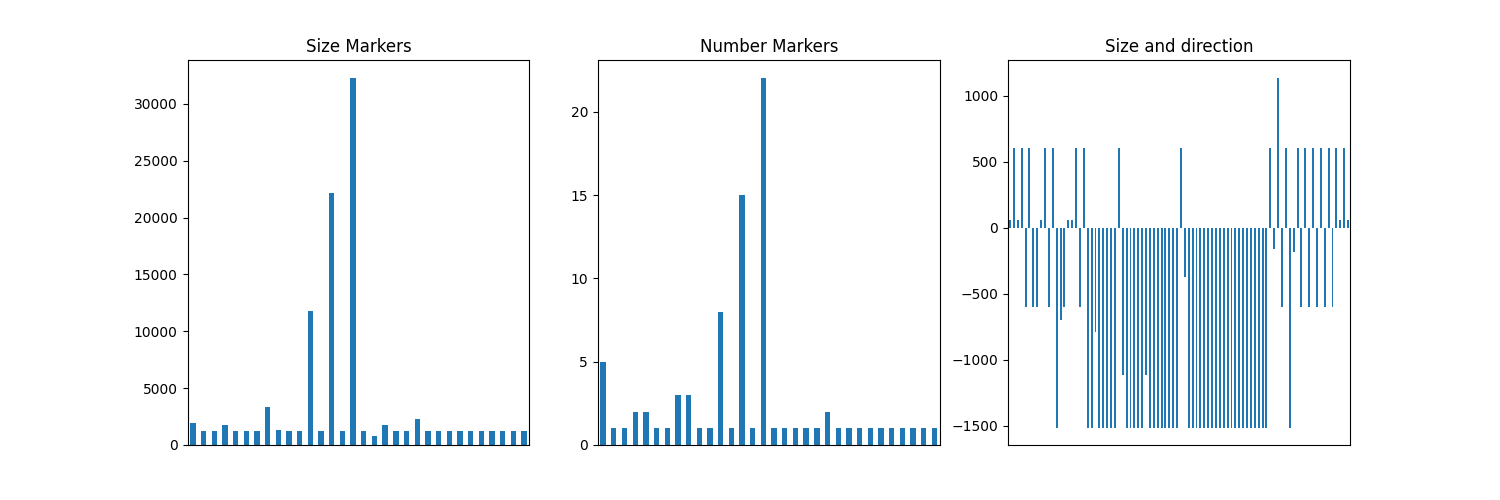
\includegraphics[width=\textwidth]{../img/facebook-figure.png}
        
\includegraphics[width=0.5\textwidth]{../img/questionMark.png}
      \end{center}
    \end{column}
    \begin{column}{0.33\textwidth}
      \begin{center}
        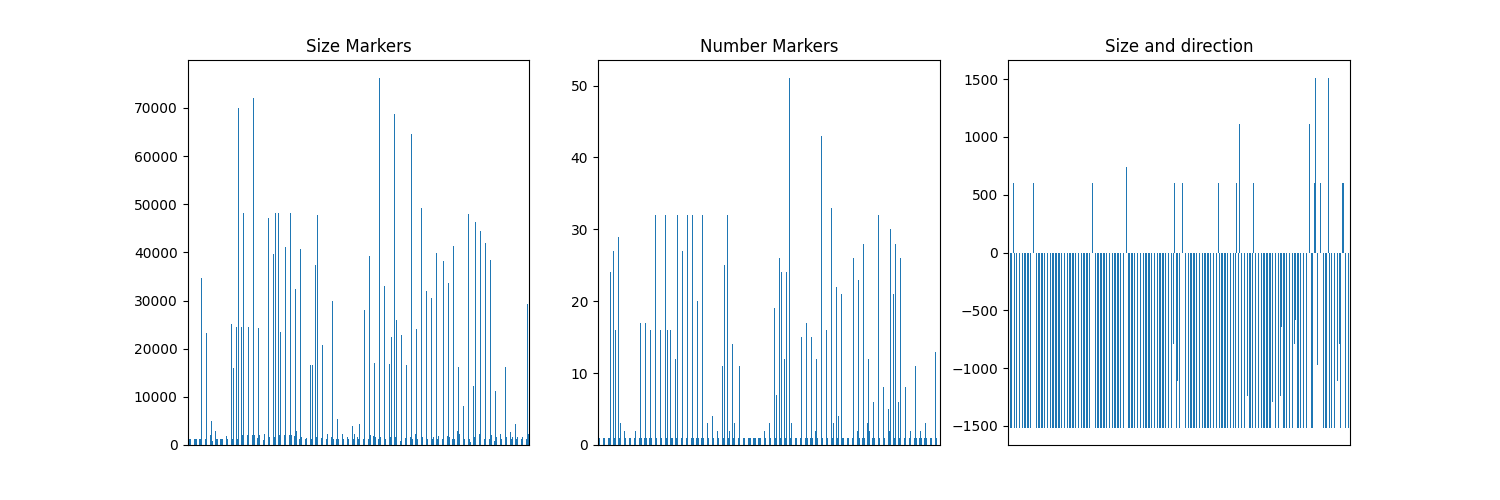
\includegraphics[width=\textwidth]{../img/unical-figure.png}
        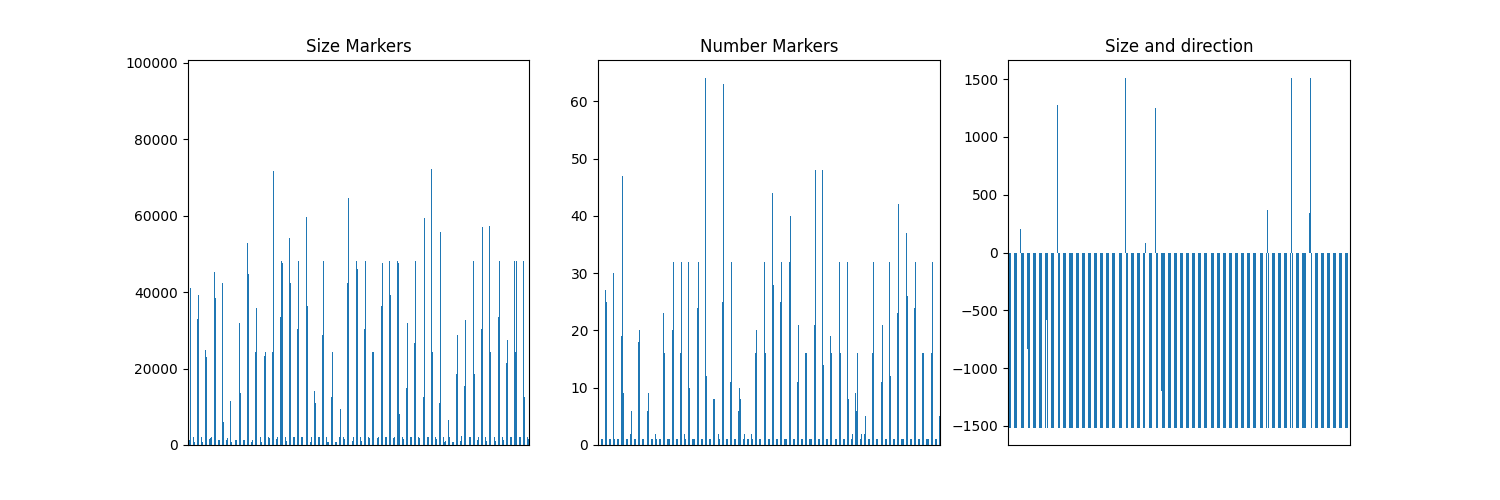
\includegraphics[width=\textwidth]{../img/youtube-figure.png}
      \end{center}
    \end{column}
  \end{columns}
\end{frame}

\begin{frame}
  \frametitle{Confronti 2}
  \begin{figure}
    \centering
    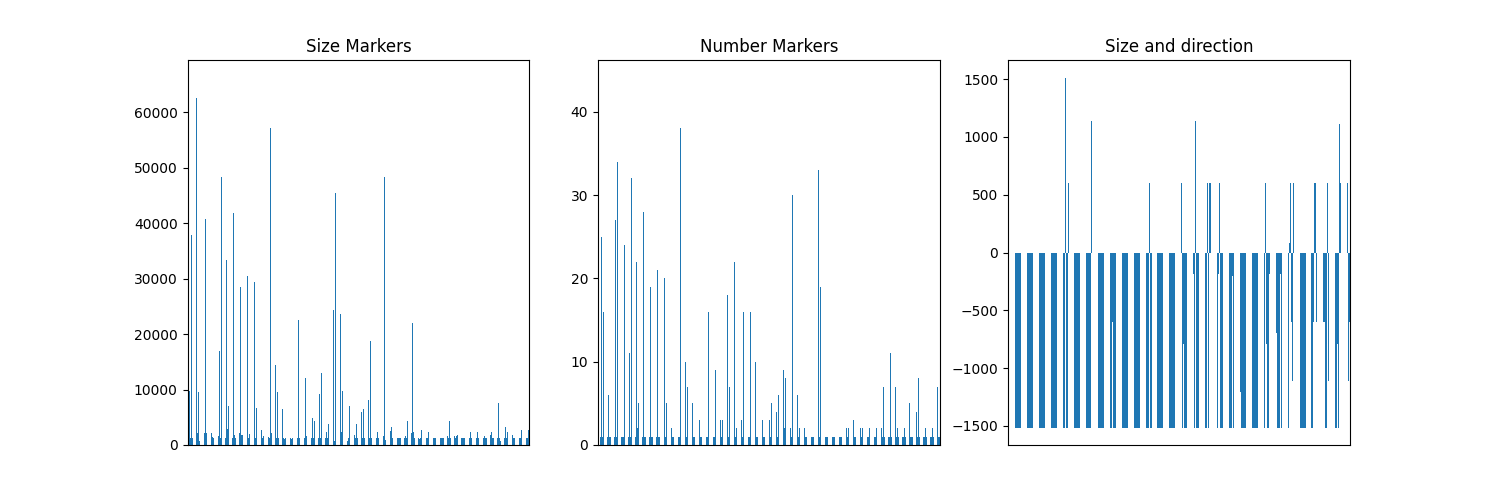
\includegraphics[width=0.851\textwidth]{../img/random-figure.png}
  \end{figure}
\end{frame}


%% \begin{frame}
%%   \frametitle{Nuova slide}
%%
%% \end{frame}
%% 
%% 
%% \begin{frame}[fragile]
%%   \frametitle{Nuova slide Codice embeddato}
%% 
%%   \begin{lstlisting}[language=Python]
%%     import numpy as np
%%     def incmatrix(genl1,genl2):
%%         m = len(genl1)
%%         n = len(genl2)
%%         M = None #to become the incidence matrix
%%         VT = np.zeros((n*m,1), int)  #dummy variable        
%%     \end{lstlisting}
%% \end{frame}
%% 
%% 
%% \begin{frame}[fragile]
%%   \frametitle{Nuova slide Codice importato}
%%   \lstinputlisting[language=sh]{../src/creazioneLab/torNetwork/host/realy.sh}
%% \end{frame}
\end{document}